\documentclass[preprint,12pt,aps,pra,showkeys,amsmath,amssymb,superscriptaddress,floatfix]{revtex4-2}
\usepackage[T1]{fontenc}
\usepackage[utf8]{inputenc}
\usepackage{amsmath,amssymb,amsthm,mathtools,mathrsfs}
\usepackage{microtype,booktabs,enumitem}
\usepackage{xcolor,tikz,etoolbox}
\usepackage[skins,breakable]{tcolorbox}
\usepackage{needspace}
% Keep diagram geometry independent of REVTeX preprint body spacing.
\AtBeginEnvironment{tikzpicture}{\linespread{1}\selectfont}
\usetikzlibrary{arrows.meta,positioning,calc,fit,decorations.pathreplacing}
\usepackage{graphicx}
\usepackage{hyperref}

\definecolor{MMBlue}{RGB}{0,82,155}
\definecolor{MMOrange}{RGB}{200,80,0}
\tikzset{
 mmnode/.style={draw=MMBlue,rounded corners=2pt,fill=MMBlue!4,align=left,execute at begin node={\raggedright},text width=5cm,font=\fontsize{10}{12}\selectfont,inner sep=6pt},
 mmimport/.style={mmnode,draw=black!65,fill=black!4},
 mmcandidate/.style={mmnode,draw=MMOrange,dashed,fill=MMOrange!5},
 mmrejected/.style={mmnode,draw=black,densely dotted,fill=black!8},
 mmproof/.style={->,thick,MMBlue},
 mmflow/.style={->,semithick,black!70},
 mmrepair/.style={->,dashed,thick,MMOrange},
 mmcandidatearrow/.style={->,dashed,semithick,MMOrange},
 mmnote/.style={font=\scriptsize,fill=white,inner sep=2pt,align=center}}

\usepackage[section]{placeins}
\setlength{\emergencystretch}{3em}
\setlist{itemsep=3pt,topsep=4pt}
\newtheorem{theorem}{Theorem}[section]
\newtheorem{proposition}[theorem]{Proposition}
\newtheorem{lemma}[theorem]{Lemma}
\newtheorem{corollary}[theorem]{Corollary}
\theoremstyle{definition}
\newtheorem{definition}[theorem]{Definition}
\newtheorem{example}[theorem]{Example}
\theoremstyle{remark}
\newtheorem{remark}[theorem]{Remark}
% Avoid isolated statement headings and single-line paragraph fragments.
\BeforeBeginEnvironment{theorem}{\Needspace{6\baselineskip}}
\BeforeBeginEnvironment{definition}{\Needspace{5\baselineskip}}
\BeforeBeginEnvironment{proposition}{\Needspace{5\baselineskip}}
\BeforeBeginEnvironment{lemma}{\Needspace{5\baselineskip}}
\BeforeBeginEnvironment{corollary}{\Needspace{5\baselineskip}}
\clubpenalty=5000
\widowpenalty=5000
\newcommand{\R}{\mathbb R}\newcommand{\Z}{\mathbb Z}\newcommand{\N}{\mathbb N}
\newcommand{\Pa}{\operatorname{Pa}}\newcommand{\Desc}{\operatorname{Desc}}
\newcommand{\cl}{\operatorname{cl}}\newcommand{\cost}{\operatorname{cost}}
\newcommand{\status}{\operatorname{status}}
% Faculty cards: a visual rail groups the five faculties within one agent.
% The rail has no arrowhead and does not represent a proof dependency.
\newcommand{\mmfacultybadge}[1]{%
 \node[circle,draw=MMBlue,line width=1pt,fill=white,
 minimum size=7mm,inner sep=0pt,font=\sffamily\small\bfseries,text=MMBlue]
 at ([xshift=15pt,yshift=-15pt]frame.north west) {#1};}
\newcommand{\mmfacultyrail}{%
 \draw[MMBlue!80,line width=1pt]
 ([xshift=15pt,yshift=2pt]frame.north west)--
 ([xshift=15pt,yshift=-2pt]frame.south west);}
\newtcolorbox{mmfacultybox}[2]{enhanced,breakable,
 colback=MMBlue!4,colframe=MMBlue!4,boxrule=0pt,arc=3pt,
 left=39pt,right=9pt,top=4pt,bottom=4pt,
 before skip=2pt,after skip=2pt,
 fontupper=\small\linespread{1.1}\selectfont,
 overlay unbroken={\mmfacultyrail\mmfacultybadge{#1}},
 overlay first={\mmfacultyrail\mmfacultybadge{#1}},
 overlay middle={\mmfacultyrail},overlay last={\mmfacultyrail}}
\newcommand{\mmfaculty}[3]{%
 \begin{mmfacultybox}{#1}{#2}
 {\sffamily\bfseries\color{MMBlue}#2}\par\smallskip #3
 \end{mmfacultybox}}
\newcommand{\agent}[9]{%
 \Needspace{8\baselineskip}
 \subsubsection{#1}
 \noindent\textbf{Object.} #2\par
 \noindent\textbf{Role.} #3\par\smallskip
 \mmfaculty{E}{Ego}{#4}
 \mmfaculty{M}{Memory}{#5}
 \mmfaculty{I}{Intellect}{#6}
 \mmfaculty{S}{Sense}{#7}
 \mmfaculty{A}{Action}{#8}
 \smallskip\noindent #9\par}

\usepackage{longtable,array,calc}
\providecommand{\tightlist}{\setlength{\itemsep}{2pt}\setlength{\parskip}{0pt}}
\makeatletter
\def\frontmatter@abstract@produce{\par\addvspace{\frontmatter@preabstractspace}%
\begingroup\prep@absbox\unvbox\absbox\post@absbox\endgroup
\addvspace{\frontmatter@postabstractspace}}
\makeatother
\newcommand{\field}[2]{\par\smallskip\noindent\textbf{#1.} #2\par}
\setlength{\emergencystretch}{5em}
\AtBeginEnvironment{verbatim}{\small\linespread{1.0}\selectfont}


\hypersetup{colorlinks=true,linkcolor=MMBlue,urlcolor=MMBlue,pdfauthor={Dibakar Sigdel}}

\begin{document}

\title{Plancherel Theorem on the Real Line\\[4pt]\large An End-to-End Meta-Math Walkthrough}

\author{Dibakar Sigdel}

\affiliation{Mindverse Computing LLC, Lynnwood, WA 98087, USA}

\date{October 2026}

\begin{abstract}

A complete authored walkthrough of plancherel theorem on the real line,
with explicit mathematical contracts, local verification gates, and
reusable exports. The report presents the target theorem, declared
imports, a dependency graph, five-faculty node contracts, a continuous
proof, a worked example, and a hypothesis-repair audit. It is an
authored mathematical exposition, not a deployed-agent transcript or a
formal proof-assistant certificate.

\end{abstract}\maketitle\linespread{1.12}\selectfont

\noindent\textbf{HA-04 / Harmonic Analysis / Report v1}

\section{Target and import contract}

\begin{theorem}

With \(\widehat f(\xi)=\int_{\mathbb R}f(x)e^{-2\pi ix\xi}\,dx\) on
Schwartz functions, prove the transform extends uniquely to a unitary
map on \(L^2(\mathbb R)\) preserving the \(L^{2}\) norm.

\end{theorem}

\subsection{Foundations and permitted imports}

A Schwartz function and all its derivatives decay faster than every
power. Import Fourier inversion on \(S(R)\) with convention
\(\widehat f(\xi )=\int f(x)e^{(-2\pi ix\xi )}dx\):
\(f(x)=\int \widehat f(\xi )e^{(2\pi ix\xi )}d\xi\). The transform and
inverse preserve S, proved by differentiation and integration by parts.
Schwartz functions are dense in \(L^{2}(R)\); \(L^{2}\) is complete.
These are substantial supporting modules, explicitly imported rather
than inferred from norm preservation.

Fubini is used only after the absolute-integrability bound
\(\|f\|_1\|\widehat h\|_1<\infty\).

\clearpage\section{Node interaction workflow}

\begin{center}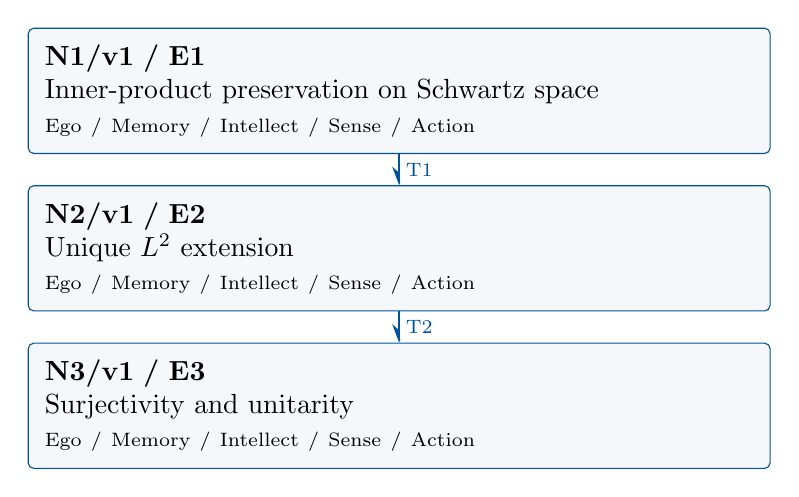
\begin{tikzpicture}[>=Stealth,x=1cm,y=1cm]

\node[mmnode,text width=9cm,minimum height=1.25cm] (N1) at (0,0.0) {\textbf{N1/v1 / E1}\\Inner-product preservation on Schwartz space\\{\scriptsize Ego / Memory / Intellect / Sense / Action}};

\node[mmnode,text width=9cm,minimum height=1.25cm] (N2) at (0,-2.0) {\textbf{N2/v1 / E2}\\Unique \(L^{2}\) extension\\{\scriptsize Ego / Memory / Intellect / Sense / Action}};

\node[mmnode,text width=9cm,minimum height=1.25cm] (N3) at (0,-4.0) {\textbf{N3/v1 / E3}\\Surjectivity and unitarity\\{\scriptsize Ego / Memory / Intellect / Sense / Action}};

\draw[mmproof] (N1.south) -- node[mmnote,right] {T1} (N2.north);

\draw[mmproof] (N2.south) -- node[mmnote,right] {T2} (N3.north);

\end{tikzpicture}\end{center}

Each box is one mathematical agent containing all five faculties. Blue
arrows carry the versioned exports listed below. The layout gives a
reading order; only drawn arrows assert dependencies. Diagnostic repair
is separate from the proof DAG.

\subsection{Versioned evidence-transfer ledger}

\begingroup\small\linespread{1.05}\selectfont

\Needspace{5\baselineskip}\field{T1: N1/E1/v1 to N2}{The Fourier transform preserves inner products and norms on S.}

\field{Receiving activity}{N2: Unique \(L^{2}\) extension}

\field{Compatibility}{Use the same mathematical objects and hypotheses as the source export.
Receiving contract: Schwartz density and norm preservation; prior
exports E1/v1}

\Needspace{5\baselineskip}\field{T2: N2/E2/v1 to N3}{A unique linear isometric extension \(U:L^{2}\to L^{2}\) with closed
range.}

\field{Receiving activity}{N3: Surjectivity and unitarity}

\field{Compatibility}{Use the same mathematical objects and hypotheses as the source export.
Receiving contract: Inversion on S and closed range; prior exports E2/v1}

\endgroup

\clearpage\section{Agent roles and five-faculty activities}\begingroup\small\linespread{1.05}\selectfont\setlist{itemsep=1pt,topsep=2pt}

\subsection{N1/v1: Inner-product preservation on Schwartz space}

\field{Object and role}{Use inversion before extending the transform.}

\field{Inputs}{\(f,h\in S\); inversion and absolute integrability; foundational imports
stated in §1}

\mmfaculty{E}{Ego}{Own E1/v1: The Fourier transform preserves inner products and norms on
S.}

\mmfaculty{M}{Memory}{Retain \(f,h\in S\); inversion and absolute integrability; foundational
imports stated in §1; keep their assumptions and versions attached.}

\mmfaculty{I}{Intellect}{Use inversion before extending the transform.}

\mmfaculty{S}{Sense}{Absolute integrability for Fubini is checked on this domain.}

\mmfaculty{A}{Action}{Carry out the numbered deductions and publish E1/v1 together with its
hypotheses and proof location.}

\smallskip\noindent\textbf{Numbered mathematical activities}

\begin{enumerate}[label=N1.\arabic*,leftmargin=3.4em]

\item Inversion for h and conjugation give
\(\operatorname{conj} (h(x))=\int \operatorname{conj} (\widehat h(\xi ))e^{(-2\pi ix\xi )}d\xi\).

\item Since \(\Vert f\Vert _{1}\Vert \widehat h\) \(\Vert _{1}<\infty\),
Fubini applies to its product with \(f(x)\).

\item Thus
\(\int f(x)\operatorname{conj} (h(x))dx=\int [\int f(x)e^{(-2\pi ix\xi )}dx]\operatorname{conj} (\widehat h(\xi ))d\xi =\int \widehat f(\xi )\operatorname{conj} (\widehat h(\xi ))d\xi\).

\item Taking \(h=f\) proves \(\Vert \widehat f\)
\(\Vert _{2}=\Vert f\Vert _{2}\) on S.

\end{enumerate}

\field{Export E1/v1}{The Fourier transform preserves inner products and norms on S.}

\field{Acceptance gate}{Absolute integrability for Fubini is checked on this domain. Publish
only after checking every displayed deduction.}

\field{Targeted repair}{If the check fails, revise N1: Absolute integrability for Fubini is
checked on this domain. Recheck dependent nodes N2, N3.}

\clearpage

\subsection{N2/v1: Unique \(L^{2}\) extension}

\field{Object and role}{Complete the isometry without using a pointwise integral for every
\(L^{2}\) function.}

\field{Inputs}{Schwartz density and norm preservation; prior exports E1/v1}

\mmfaculty{E}{Ego}{Own E2/v1: A unique linear isometric extension \(U:L^{2}\to L^{2}\) with
closed range.}

\mmfaculty{M}{Memory}{Retain Schwartz density and norm preservation; prior exports E1/v1; keep
their assumptions and versions attached.}

\mmfaculty{I}{Intellect}{Complete the isometry without using a pointwise integral for every
\(L^{2}\) function.}

\mmfaculty{S}{Sense}{\(L^{2}\) equivalence classes do not necessarily have an absolutely
convergent Fourier integral.}

\mmfaculty{A}{Action}{Carry out the numbered deductions and publish E2/v1 together with its
hypotheses and proof location.}

\smallskip\noindent\textbf{Numbered mathematical activities}

\begin{enumerate}[label=N2.\arabic*,leftmargin=3.4em]

\item For \(f\in L^{2}\) choose \(f_j\in S\) with \(f_j\to f\) in \(L^{2}\).

\item The norm identity makes \(\widehat f_j\) Cauchy, so it converges to an
\(L^{2}\) element Uf.

\item A second approximating sequence gives the same limit by
\(\Vert \widehat f_j-\widehat g_j\Vert _{2}=\Vert f_j-g_j\Vert _{2}\).

\item This defines a linear isometry extending the transform, uniquely because
S is dense.

\item Its range is closed: a convergent sequence \(Uf_j\) makes \(f_j\)
Cauchy, and its limit maps to the given range limit.

\end{enumerate}

\field{Export E2/v1}{A unique linear isometric extension \(U:L^{2}\to L^{2}\) with closed
range.}

\field{Acceptance gate}{\(L^{2}\) equivalence classes do not necessarily have an absolutely
convergent Fourier integral. Publish only after checking every displayed
deduction.}

\field{Targeted repair}{If the check fails, revise N2: \(L^{2}\) equivalence classes do not
necessarily have an absolutely convergent Fourier integral. Recheck
dependent nodes N3.}

\clearpage

\subsection{N3/v1: Surjectivity and unitarity}

\field{Object and role}{Show the range contains a dense subset.}

\field{Inputs}{Inversion on S and closed range; prior exports E2/v1}

\mmfaculty{E}{Ego}{Own E3/v1: The transform extends uniquely to a unitary \(L^{2}\) map.}

\mmfaculty{M}{Memory}{Retain Inversion on S and closed range; prior exports E2/v1; keep their
assumptions and versions attached.}

\mmfaculty{I}{Intellect}{Show the range contains a dense subset.}

\mmfaculty{S}{Sense}{Isometry alone does not imply onto; use dense range plus closedness.}

\mmfaculty{A}{Action}{Carry out the numbered deductions and publish E3/v1 together with its
hypotheses and proof location.}

\smallskip\noindent\textbf{Numbered mathematical activities}

\begin{enumerate}[label=N3.\arabic*,leftmargin=3.4em]

\item Every \(g\in S\) is the transform of its Schwartz inverse transform;
hence S lies in the range of U.

\item The range is closed and contains dense S, so it is all \(L^{2}\).

\item Inner-product preservation passes from Schwartz approximations to
\(L^{2}\) limits.

\item Thus U is unitary with its inverse obtained by the same completion of
the inverse transform.

\end{enumerate}

\field{Export E3/v1}{The transform extends uniquely to a unitary \(L^{2}\) map.}

\field{Acceptance gate}{Isometry alone does not imply onto; use dense range plus closedness.
Publish only after checking every displayed deduction.}

\field{Targeted repair}{If the check fails, revise N3: Isometry alone does not imply onto; use
dense range plus closedness. Withhold this terminal result until its
gate passes.}

\endgroup\clearpage\section{Continuous mathematical proof}\label{sec:proof}

Read these steps in order as one proof; the diagram is optional.
Numbered activities identify the specific constructions and deductions
owned by each node.

\subsection{§4.N1 --- Inner-product preservation on Schwartz
space}\label{n1-inner-product-preservation-on-schwartz-space}

\begin{enumerate}
\def\labelenumi{\arabic{enumi}.}
\item
  Inversion for h and conjugation give
  \(\operatorname{conj} (h(x))=\int \operatorname{conj} (\widehat h(\xi ))e^{(-2\pi ix\xi )}d\xi\).
\item
  Since \(\Vert f\Vert _{1}\Vert \widehat h\) \(\Vert _{1}<\infty\),
  Fubini applies to its product with \(f(x)\).
\item
  Thus
  \(\int f(x)\operatorname{conj} (h(x))dx=\int [\int f(x)e^{(-2\pi ix\xi )}dx]\operatorname{conj} (\widehat h(\xi ))d\xi =\int \widehat f(\xi )\operatorname{conj} (\widehat h(\xi ))d\xi\).
\item
  Taking \(h=f\) proves \(\Vert \widehat f\)
  \(\Vert _{2}=\Vert f\Vert _{2}\) on S.
\end{enumerate}

\subsection{\texorpdfstring{§4.N2 --- Unique \(L^{2}\)
extension}{§4.N2 --- Unique L\^{}\{2\} extension}}\label{n2-unique-l2-extension}

\begin{enumerate}
\def\labelenumi{\arabic{enumi}.}
\item
  For \(f\in L^{2}\) choose \(f_j\in S\) with \(f_j\to f\) in \(L^{2}\).
\item
  The norm identity makes \(\widehat f_j\) Cauchy, so it converges to an
  \(L^{2}\) element Uf.
\item
  A second approximating sequence gives the same limit by
  \(\Vert \widehat f_j-\widehat g_j\Vert _{2}=\Vert f_j-g_j\Vert _{2}\).
\item
  This defines a linear isometry extending the transform, uniquely
  because S is dense.
\item
  Its range is closed: a convergent sequence \(Uf_j\) makes \(f_j\)
  Cauchy, and its limit maps to the given range limit.
\end{enumerate}

\subsection{§4.N3 --- Surjectivity and
unitarity}\label{n3-surjectivity-and-unitarity}

\begin{enumerate}
\def\labelenumi{\arabic{enumi}.}
\item
  Every \(g\in S\) is the transform of its Schwartz inverse transform;
  hence S lies in the range of U.
\item
  The range is closed and contains dense S, so it is all \(L^{2}\).
\item
  Inner-product preservation passes from Schwartz approximations to
  \(L^{2}\) limits.
\item
  Thus U is unitary with its inverse obtained by the same completion of
  the inverse transform.
\end{enumerate}

\hfill$\square$

\section{Worked orchestration}

For \(f(x)=e^{(-\pi x^{2})}\), the Gaussian integral calculation gives
\(\widehat f=f\) under this convention. Both squared norms equal
\(\int e^{(-2\pi x^{2})}dx=1/\sqrt{2}\). The inverse phase has the
opposite sign; \(retaining2\pi\) avoids an erroneous normalization
factor.

\subsection{Boundary and hypothesis audit}

The \(function(1+|x|)^{(-3/4)}\) belongs to \(L^{2}\) but notL \(^{1}\).
Its Fourier transform is defined by completion, not an absolutely
convergent integral at every frequency. Sense rejects a
pointwise-integral export for all \(L^{2}\) inputs and retains the
equivalence-class contract.

\section{Illustrative failure and repair}

The following is an authored diagnostic scenario. Changed assumptions
define a new contract; they do not retroactively prove the original
statement.

\subsection{Failure and correction}
This is an authored teaching trace, not a recorded agent run.

\begin{enumerate}
\def\labelenumi{\arabic{enumi}.}
\tightlist
\item
  \textbf{Ego \(\to\) Memory:} register the §1 theorem, imports, and
  requested exports before beginning the proof.
\item
  \textbf{Intellect \(\to\) Action:} choose the bridges in §3 and carry
  out the numbered activities in §4; transmit only established E-exports
  along the §2 DAG.
\item
  \textbf{Sense \(\to\) responsible node:} test the specific
  boundary/failure in §5 and the node's individual audit. A failing
  candidate is withheld; downstream nodes may not use it.
\item
  \textbf{Memory + Intellect:} identify whether the error is an omitted
  condition, an invalid inference, or an attempted extension beyond the
  theorem. Restore the exact contract or explicitly state a different
  one.
\item
  \textbf{Action:} redo the affected mathematical activity using the
  repaired condition or inference. Recheck consuming nodes, rather than
  feeding their conclusions back as premises.
\item
  \textbf{Ego:} publish only the supported export with its assumptions
  and proof location. A hypothetical revised export is v2; the written
  proof here is the v1 exposition, not a claim that this repair was
  executed.
\end{enumerate}

\subsection{Hypothesis boundary}
The \(function(1+|x|)^{(-3/4)}\) belongs to \(L^{2}\) but notL \(^{1}\).
Its Fourier transform is defined by completion, not an absolutely
convergent integral at every frequency. Sense rejects a
pointwise-integral export for all \(L^{2}\) inputs and retains the
equivalence-class contract.

\subsection{Version and recheck}
Treat any changed assumption as a new contract. Recheck the revised
export and all of its descendants. A backward diagnostic never
establishes an earlier theorem. This is an authored teaching trace, not
an execution log.

\par\medskip\begingroup\small\linespread{1.0}\selectfont\noindent\textbf{Provenance.} This authored proof is complete relative to its declared imports. Reuse
each export with its assumptions, proof, and version. The original
Markdown remains available for comparison.
\par\endgroup

\end{document}
